\begin{frame}[c]{In a Nutshell}

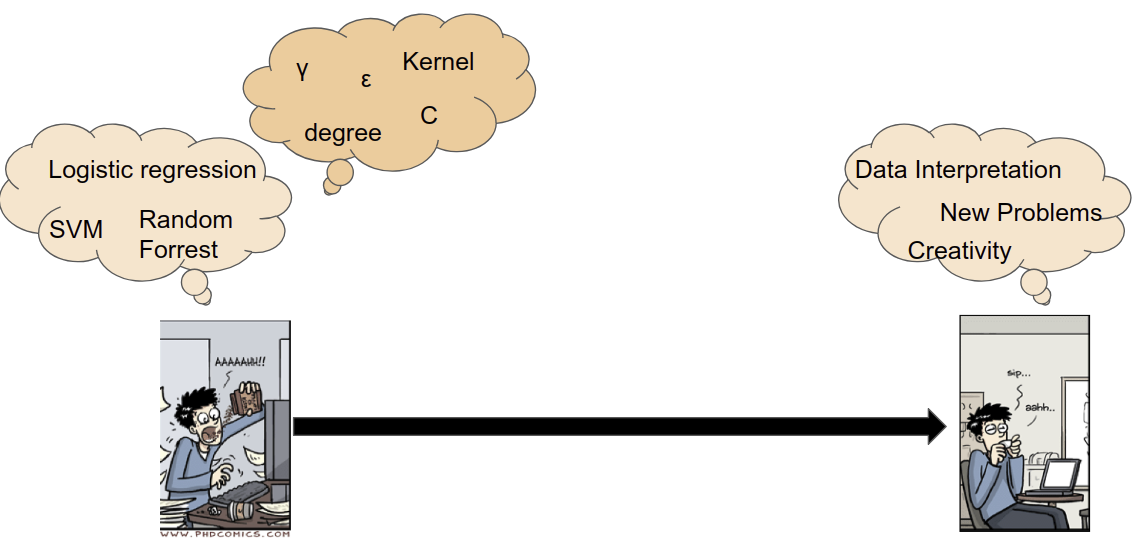
\includegraphics[width=0.99\textwidth]{images/automl_comic}

\end{frame}
%----------------------------------------------------------------------
%----------------------------------------------------------------------
\begin{frame}[c]{}

\huge
\centering
What are your expectations for the course?

\bigskip


\includegraphics[scale=0.1]{images/hands.png}

\end{frame}
%----------------------------------------------------------------------
\begin{frame}[c]{}

\centering
\huge
Lecture 1:\\
Overview and Motivation
\end{frame}
%----------------------------------------------------------------------
%----------------------------------------------------------------------
\begin{frame}[c]{Overview}

What do we learn today?

\begin{itemize}
  \item What is AutoML?
  \item \ldots
  \item Organization of the course
\end{itemize}

\end{frame}
%-----------------------------------------------------------------------
%----------------------------------------------------------------------
\begin{frame}[c]{Course Overview}

\begin{itemize}
	\item TODO
\end{itemize}


\end{frame}
%----------------------------------------------------------------------
%----------------------------------------------------------------------
\begin{frame}[c]{Team (1)}

\begin{columns}[T]
\column{0.7\textwidth}
\begin{itemize}
  \item Frank Hutter
  \item Head of machine learning lab
  \item PhD at the University of British Columbia (Canada)
  \item Background: Machine learning and combinatorial optimization
  \item Expertise in algorithm configuration, algorithm selection, automated machine learning,\ldots
\end{itemize}
\column{0.3\textwidth}
\vspace*{0.7cm}
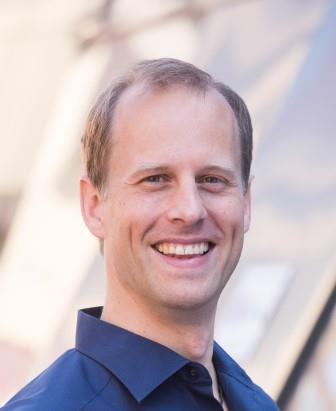
\includegraphics[width=6.7em]{images/team/frank_small}

\end{columns}

\end{frame}
%----------------------------------------------------------------------
%----------------------------------------------------------------------
\begin{frame}[c]{Team (2)}

\begin{columns}[T]
\column{0.7\textwidth}
\begin{itemize}
  \item Marius Lindauer
  \item Junior research group lead of automatic algorithm design
  \item PhD at University of Potsdam
  \item Expertise in algorithm configuration, algorithm selection and AutoML
  \item Maintainer of ASlib and AClib
 % \item Background: Hard combinatorial problems (e.g., SAT and ASP)
\end{itemize}
\column{0.3\textwidth}

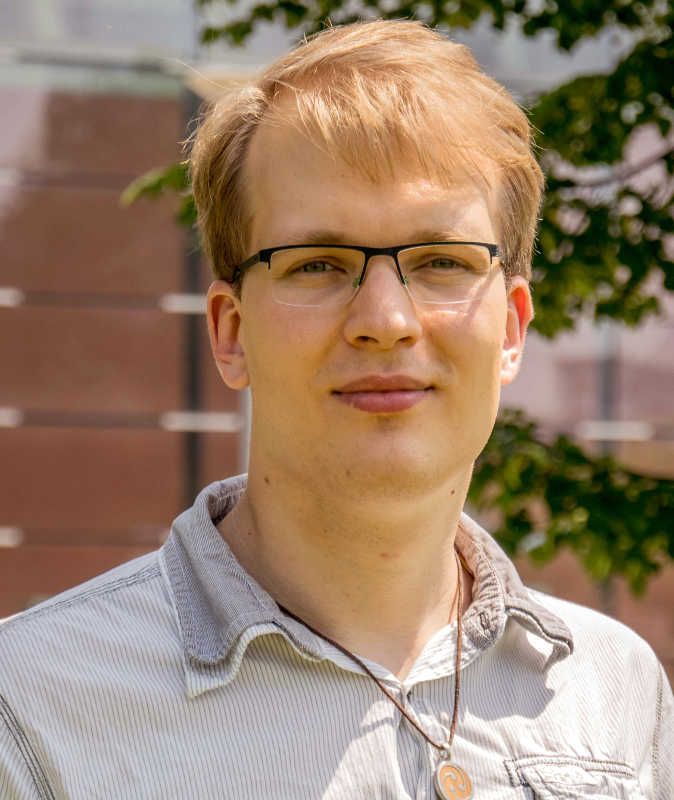
\includegraphics[width=6.7em]{images/team/marius}
\end{columns}

\end{frame}
%----------------------------------------------------------------------
%----------------------------------------------------------------------
\begin{frame}[c]{Team -- Exercise}

\begin{columns}[T]
\column{0.7\textwidth}
\begin{itemize}
  \item Andr\'e Biedenkapp
  \item PhD student
  \item Focus on algorithm control
  \item Responsible for exercises
\end{itemize}
\column{0.3\textwidth}

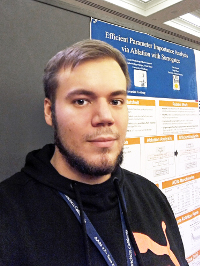
\includegraphics[width=6.7em]{images/team/biedenkapp}
\end{columns}

\end{frame}
%----------------------------------------------------------------------
%----------------------------------------------------------------------
\begin{frame}[c]{Organization (Lectures)}

\begin{itemize}
  \item $6$ ECTS
  \item Every week at Monday: 14:15 (s.t) - 15:45\\ (Building: 106 Room: SR 00 007)
  \item \emph{Interactive} Lecture 
  \item Course material on our homepage\\
  		{\small \url{ml.informatik.uni-freiburg.de/teaching/ws2018/ml4aad/}}
  \item Slides will be online before the lectures
  \item No video recording!
\end{itemize}


\end{frame}
%-----------------------------------------------------------------------
%----------------------------------------------------------------------
\begin{frame}[c]{Organization (Exercises)}

\begin{itemize}
  \item Every Tuesday at: 12:30 - 14:00\\ (Building: 051 Room: SR 00 006)
  \begin{itemize}
    \item No meeting this week, but first exercise sheet!
  \end{itemize}
  \item Roughly every week new exercise sheet and discussion of last exercise
  \item Most exercises will be practical, i.e., you have to implement something
  \item Team work allowed, max team size: 2! 
  %\item Each exercise will be worth at most $50$ points
  \item Cheating:
  \begin{itemize}
    \item First time cheating: $0$ points for exercise
    \item Second time cheating: failing the course
  \end{itemize}
  \item You have to obtain at least $50\%$ points in the exercises  
  \item Not all assignments will provide the same amount of points
  \item Submit via bitbucket (git)
\end{itemize}

\end{frame}
%-----------------------------------------------------------------------
%----------------------------------------------------------------------
% \begin{frame}[c]{Exceptions (tentative)}
% 
% \begin{itemize}
% 	\item No lectures and exercises during vacations and holidays\\ (1. Nov, 25. Dec, 27. Dec, 01. Jan, 03. Jan)
% 	\item Switching lecture and exercise slot 11. Dec and 13. Dec
% 	\item Last lecture at 05. Feb
% \end{itemize}
% 
% \end{frame}
%-----------------------------------------------------------------------
%----------------------------------------------------------------------
\begin{frame}[c]{Requirements}

\begin{itemize}
  \item Knowledge in Machine Learning (strongly recommended)
  \begin{itemize}
    \item Classification, regression, clustering, decision tree, training-test split, cross validation, deep learning \ldots
  \end{itemize}
  \pause
  \item Basic knowledge in AI 
  \begin{itemize}
    \item decision problems, optimization problems, NP-hard, \ldots 
  \end{itemize}
  \pause
  \item Experience in Python and git 
  \begin{itemize}
    \item nearly all exercises will require that you implement something in~Python and submit the solution to a git repo
  \end{itemize}
\end{itemize}

\end{frame}
%-----------------------------------------------------------------------
%----------------------------------------------------------------------
\begin{frame}[c]{Final Oral Exam}

\begin{itemize}
  \item Implement a larger project (worth $1-2$ weeks fulltime)
	\begin{itemize}
		\item No teamwork!
	\end{itemize}
  \item Exam
	\begin{itemize}
		\item Present the project in the first $15$ minutes\\ (including some questions from us)
		\item Answer questions about further course material in the second $15$ minutes
	\end{itemize}	
\end{itemize}

\end{frame}
%-----------------------------------------------------------------------
%----------------------------------------------------------------------
\begin{frame}[c]{Chances and Risks}

ML4AAD is an advanced lecture and we modify it each time.

\bigskip
\pause

Chances:
\begin{itemize}
  \item All presented topics are close to state-of-the-art;\\there is active research on these topics  
  \item The course will provide a solid background\\ for doing a master project/thesis in our group 
\end{itemize}

\medskip

Risks:
\begin{itemize}
  \item You will find some typos and issues in the slides;\\ please tell us if you find something
  %\item Workload could be very high for you -- we have no experience with the exercises yet
\end{itemize}

\medskip
\pause
$\to$ Give us some feedback and we will improve the course!

\end{frame}
%-----------------------------------------------------------------------
%----------------------------------------------------------------------
\begin{frame}[c]{Introduce yourself!}

\begin{itemize}
  \item Why have you chosen this course?
  \medskip
  \item Background knowledge? (AI, ML, \ldots)
  \medskip 
  \item Experience with such problems?
\end{itemize}

\bigskip
\centering

\includegraphics[scale=0.1]{images/hands.png}

\end{frame}
%-----------------------------------------------------------------------
%----------------------------------------------------------------------
% \begin{frame}[c]{Exercise I }
% 
% \begin{block}{Task}
% \begin{enumerate}
% 	\item Identify $2$ (known) algorithms which have tunable parameters and briefly describe these parameters
% 	\item Describe a manual way to tune the parameters and approximate the effort you would need to do this on an example
% 	\item Analyze the runtime complexity of the algorithms
% \end{enumerate}
% \end{block}
% 
% \alert{Submission due 02.11. (23:59 GMT)}\\
% Submit at ILIAS : \url{https://ilias.uni-freiburg.de/goto.php?target=crs_465155&client_id=unifreiburg}
% %Send to: \url{lindauer@cs.uni-freiburg.de}\\
% %with subject: \texttt{[MLOAD Excercise I] $<$your name$>$} 
% 
% \end{frame}
%-----------------------------------------------------------------------
% %----------------------------------------------------------------------
% \begin{frame}[c]{}
% 
% 
% 
% \end{frame}
% %-----------------------------------------------------------------------

